% %%%%%%%%%%%%%%%%%%%%%%%%%%%%%%%%%%%%%%%%%%%%%%%%%%%%%%%%%%%%%%%%%%%%%
% %% SpDCache %%
% Architecture of SpDCache
% %%%%%%%%%%%%%%%%%%%%%%%%%%%%%%%%%%%%%%%%%%%%%%%%%%%%%%%%%%%%%%%%%%%%%

\section{Architecture of SpDCache}
\label{sec:spdc:archispdc}

\lettrine{W}{e} design a specialized data-cache architecture, called \acrlong{spdc}, that exploits the two-region structure of \gls{banded} matrices to reduce memory traffic during \glspl{reduction} operations on the output vector $c$.
To better understand \acrlong{spdc} behavior, our study focuses on a single-level cache hierarchy with a single core executing \acrshort{spmv} kernels on \gls{banded} matrix case.
However, \acrlong{spdc} is designed to extend to multilevel memory hierarchies and multicore architectures (see Chapter~\ref{cha:optim}), and to adapt to other region configurations.
As an isolated data-cache, \acrlong{spdc} must satisfy three key requirements:
\begin{itemize}
    \item \textbf{Generic cache functionality:} \acrlong{spdc} operates as a standard cache for load and store instructions from the processor, enabling sequential reads of matrix $A$ and vector $b$ to leverage spatial locality.
    \item \textbf{Reduction capability:} \acrlong{spdc} functions as a \gls{redC} to minimize inherent memory traffic costs of \gls{reduction} operations on output vector $c$.
    \item \textbf{Region-wise reduction:} Dedicated cache regions for sparse and dense matrix regions mitigate the \gls{irrAccess} patterns of \glspl{reduction}.
\end{itemize}

As shown in Figure~\ref{fig:spdc:cache_partition}, \acrlong{spdc} is divided into three memory regions.
The first, \acrfull{grc}, is for all memory transactions unrelated to the output vector $c$, including reads of $A$ and $b$.
It is a classic, \gls{set}-associative cache and is required for the processor to operate normally, but is not the focus in this chapter.
The other two regions, called \acrfull{drc} and \acrfull{srt}, are able to perform \glspl{reduction} on $c$.
The \acrshort{drc} works as a line-wise, \gls{set}-associative \gls{redC} to hold high density data in the \acrlong{ibr} of the matrix (\acrshort{ibr}, \textit{orange}).
The difference with the \acrshort{grc} is that it is able to perform \glspl{reduction} and it is dedicated to the \emph{banded} region, so that spurious accesses outside of the \gls{band} do not provoke undesired \glspl{eviction}.
Finally, the \acrshort{srt} works as an element-wise, fully-associative table whose role is to handle sparse regions, such as the \acrlong{obr} in the matrix (\acrshort{obr}, \textit{blue}).
This region is well-suited for handling isolated data and reducing memory traffic, with further analysis of this design choice presented in the next chapter.

\begin{figure}[htbp]
    \centering
    \begin{minipage}[b]{0.58\linewidth}
        \begin{figure}[H]
    		\centering
    		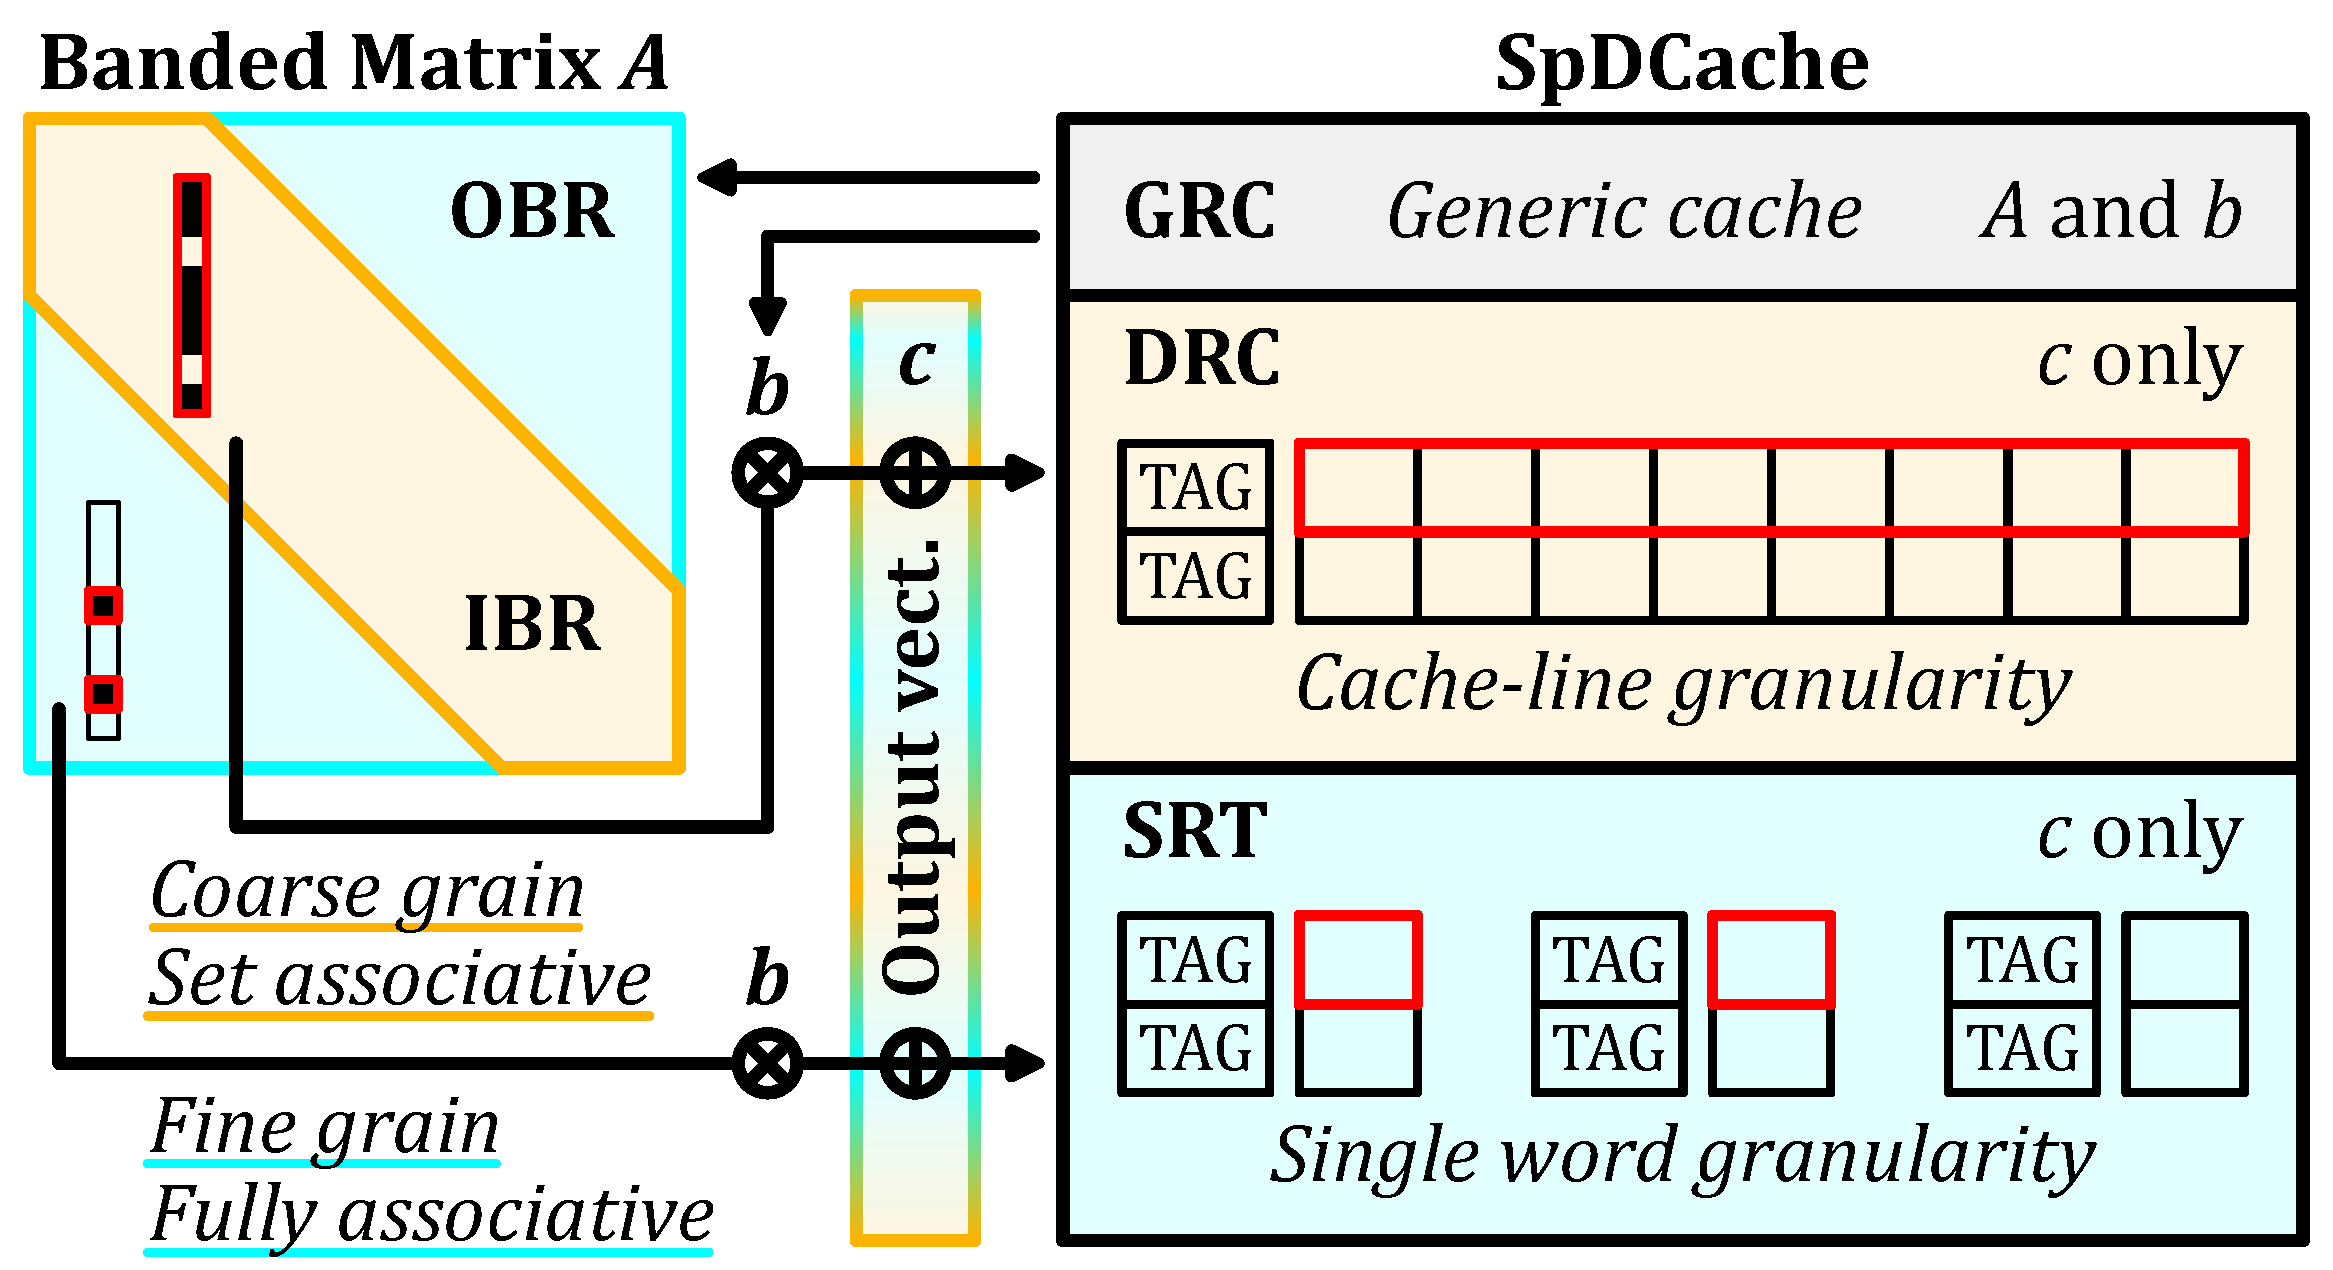
\includegraphics[width=\linewidth]{Chapter_SpDC/Figures/PDF/SpDCPartitioning.pdf}
    		\caption{Data-Cache Partitioning into Regions (\acrshort{grc}, \acrshort{drc}, \acrshort{srt})}
    		\label{fig:spdc:cache_partition}
    	\end{figure}
    \end{minipage}
    \hfill
    \begin{minipage}[b]{0.38\linewidth}
    	\begin{figure}[H]
    		\centering
    		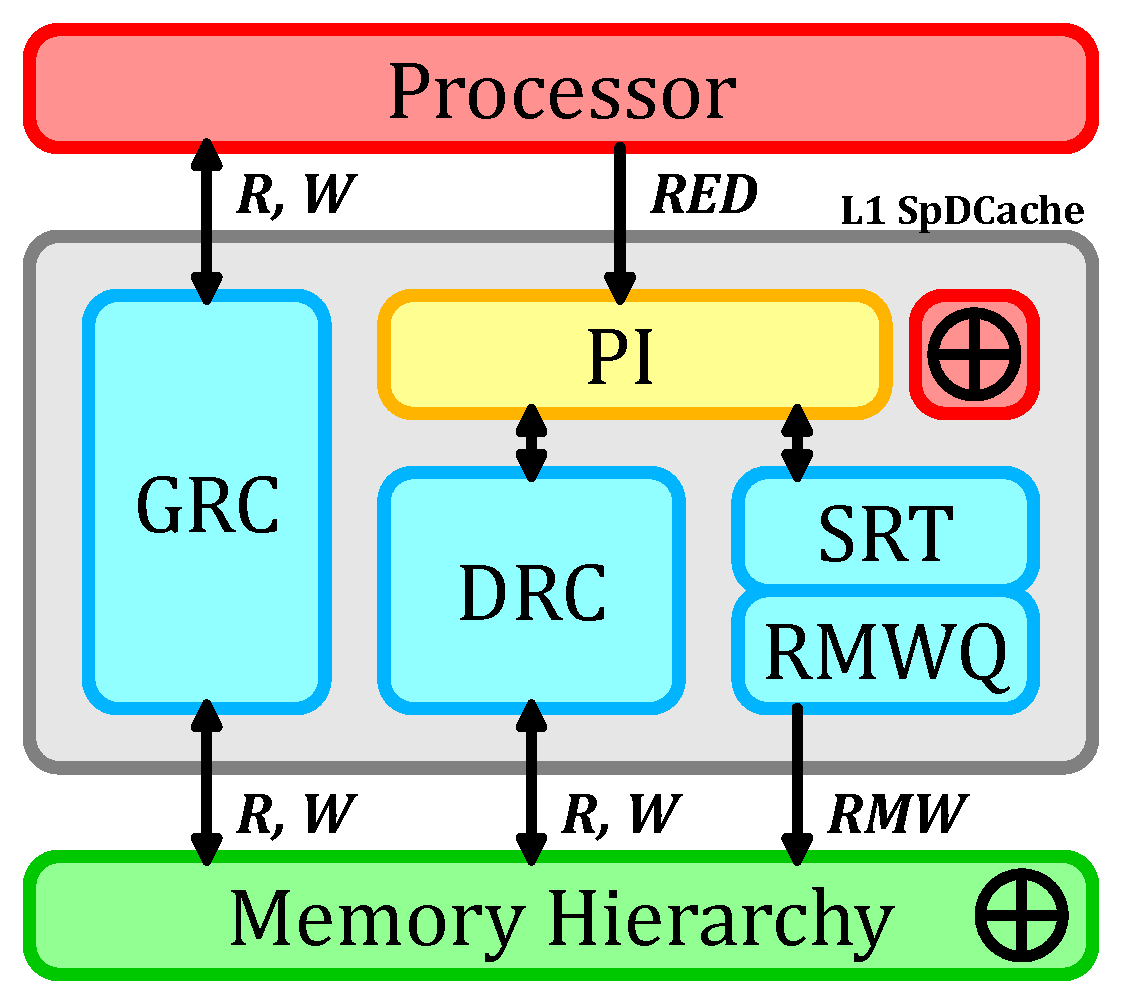
\includegraphics[width=\linewidth]{Chapter_SpDC/Figures/PDF/SpDC_MacroArchi.pdf}
    		\caption{Simplified View of the Memory Hierarchy with \acrlong{spdc}}
    		\label{fig:spdc:global_view_archi}
    	\end{figure}
    \end{minipage}
\end{figure}

Figure~\ref{fig:spdc:global_view_archi} shows a simplified view of a memory hierarchy with \acrlong{spdc}.
The \emph{Processor Interface} (\emph{PI}) takes \gls{reduction} instructions, \emph{RED(key, value, region)}, from the processor.
The \acrshort{red} instruction contains a `region' field which indicates whether the value is expected to be in a dense region (\acrshort{drc}) or a sparse region (\acrshort{srt}).
As we will see, the hardware may override the software selection to avoid duplication.
The \acrshort{drc} communicates with the memory hierarchy using read and write transactions over entire cache-lines, to propagate the local \emph{updates} to the downstream memory.
As \acrshort{srt} \emph{updates} are for isolated elements, it does not make sense to bring a full line into the L1 to modify a single word. 
The \acrshort{srt} thus propagates \emph{updates} by issuing atomic, element-wise \acrlong{rmw} transactions (\acrshortpl{rmw}), which must be processed remotely and 
close to the main memory.
This is a stringent requirement for the memory hierarchy, but it is realistic.
Indeed, existing protocols such as \mbox{AXI-4}~\cite{ARM2023_AXI} already support atomic transactions for certain operations (logical, integer add, min, max) and these could be extended to include floating point addition.
Moreover, this requirement becomes more manageable when extending \acrlong{spdc} to multilevel cache hierarchies (see Chapter~\ref{cha:optim}).
The \acrshortpl{rmw} from the \acrshort{srt} are temporarily buffered in a small queue (\acrshort{rmwq}), to avoid congestion.

\acrlong{spdc} is driven by three key design principles.
First, we ensure a given \emph{key} is in only one region at a time, to avoid coherency problems.
Second, the \acrshort{drc} is given priority over the \acrshort{srt}, to enable coalescing.
Third, we avoid bringing a full line from memory to the L1 to simply update one or a few entries.

\begin{figure}[htbp]
    \centering
    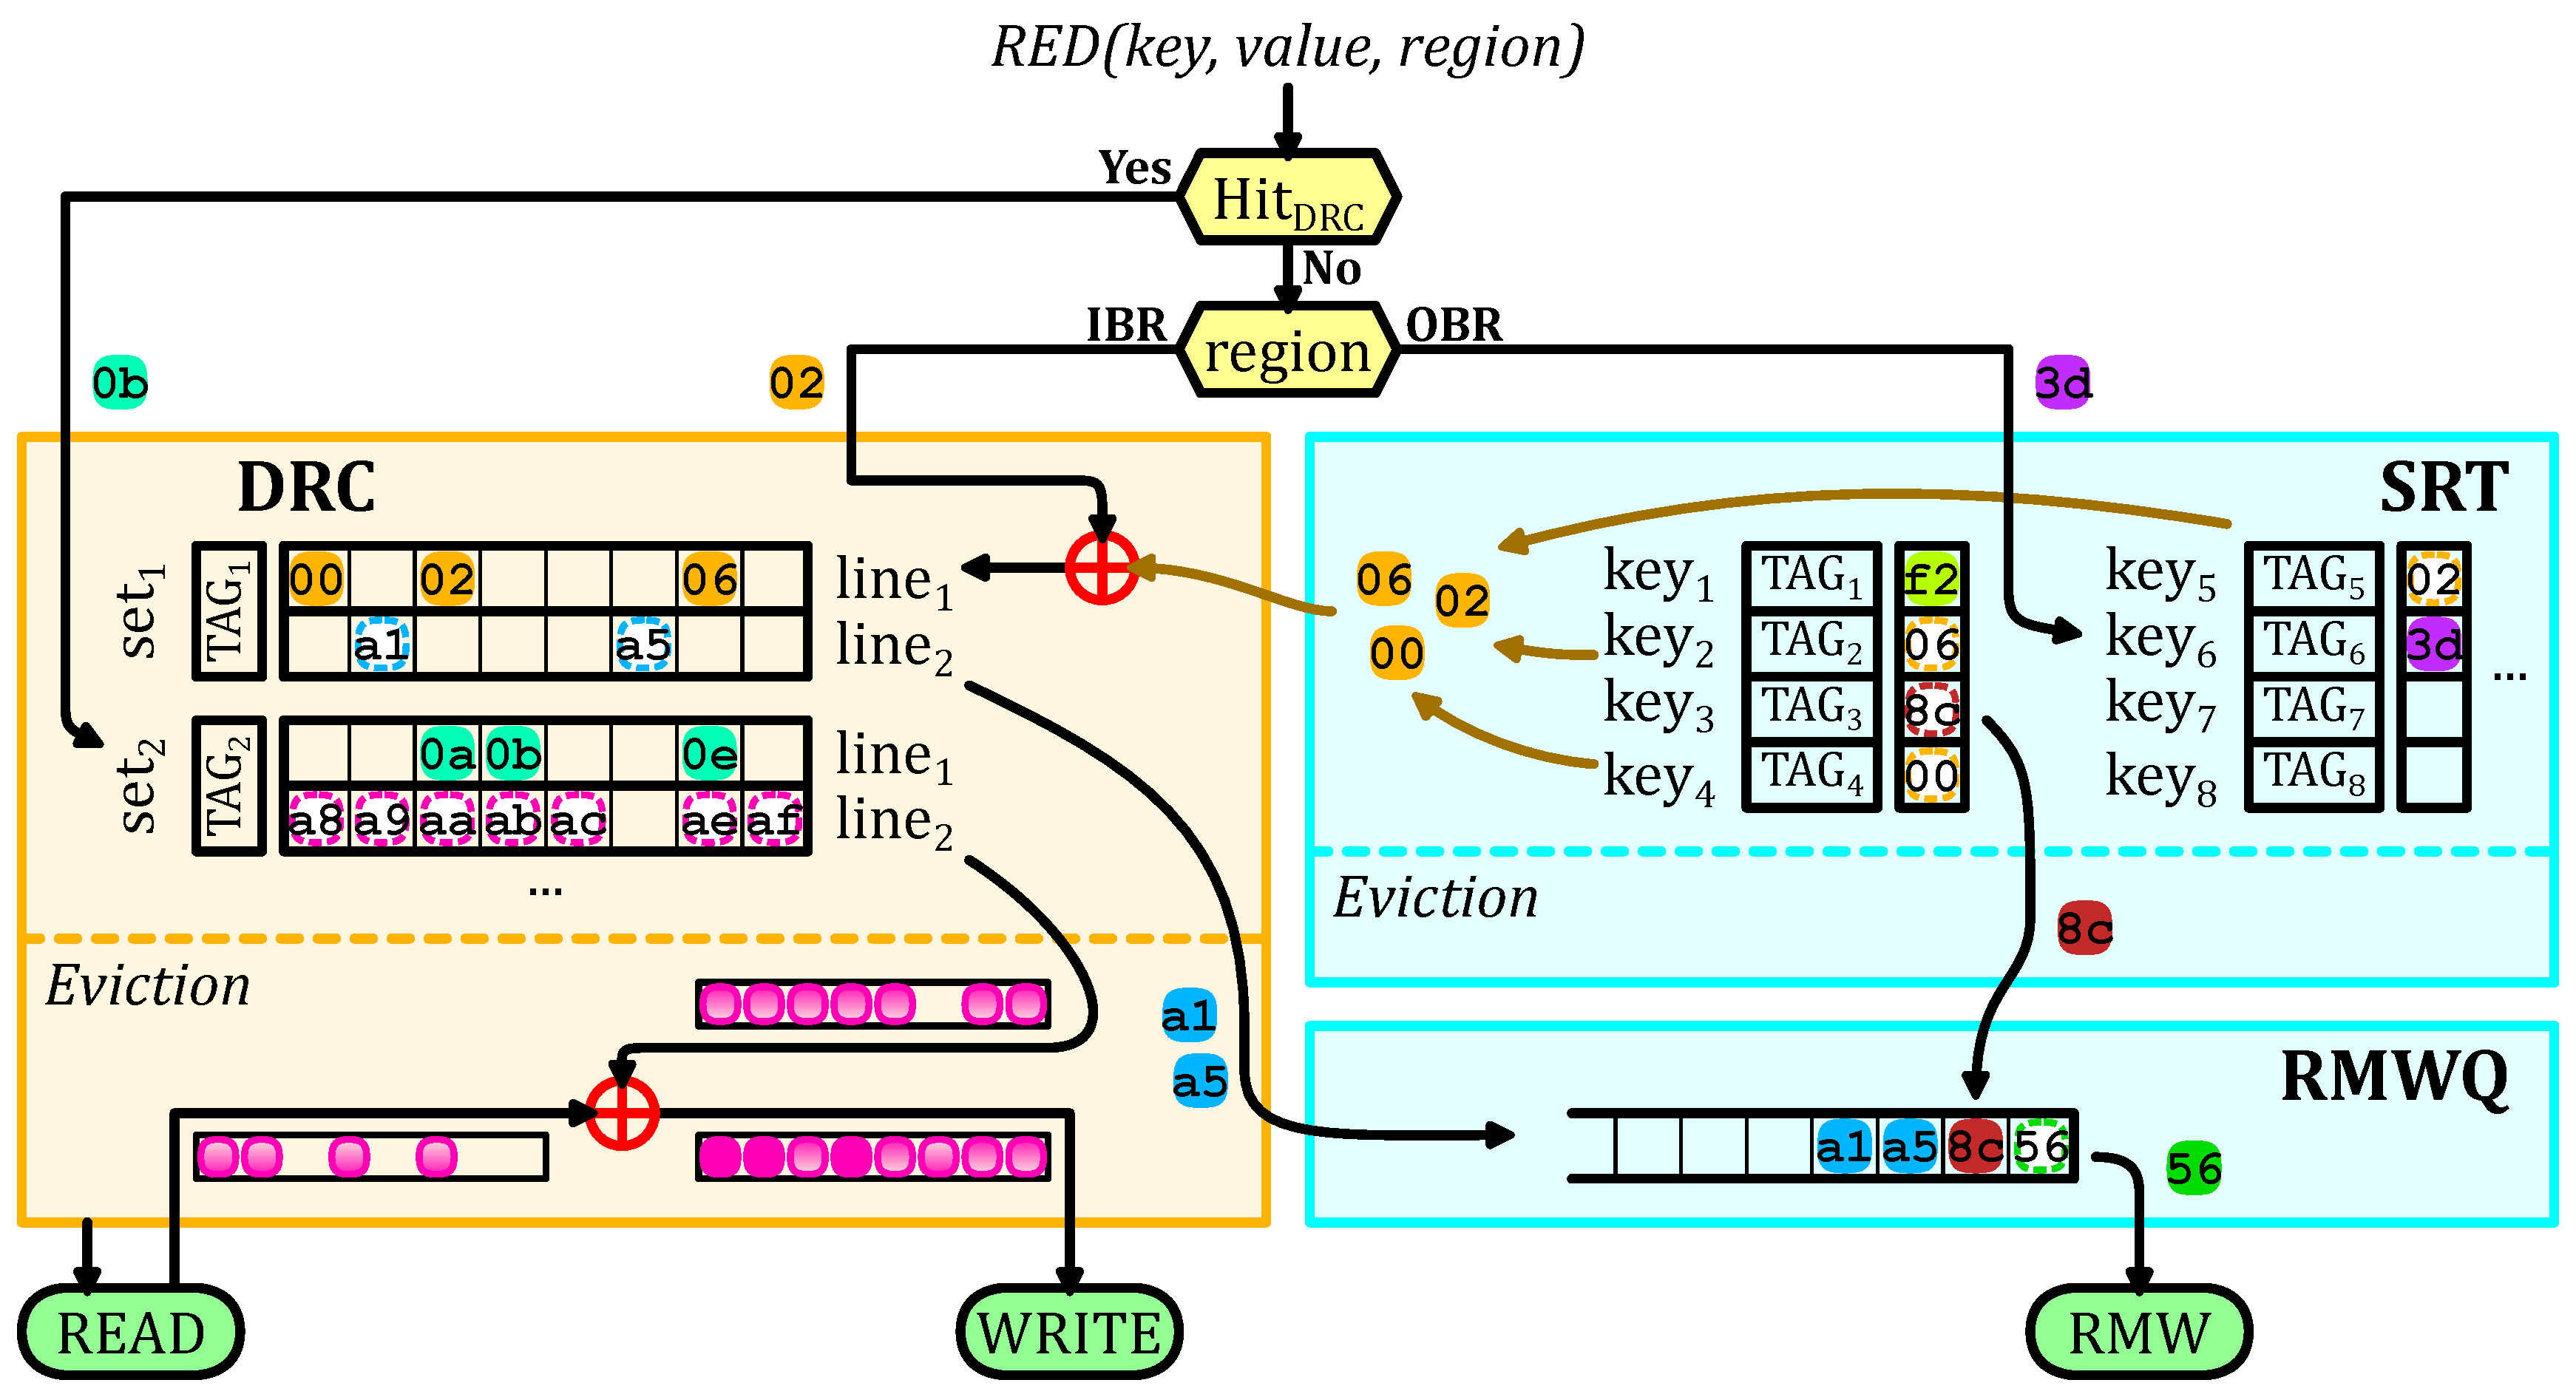
\includegraphics[width=\linewidth]{Chapter_SpDC/Figures/PDF/SpDC_behavior.pdf}
    \caption{Internal Operation of \acrlong{spdc} with Examples}
    \label{fig:spdc:spdc_archi}
\end{figure}

In Figure~\ref{fig:spdc:spdc_archi}, we describe the operation of \acrlong{spdc}, via a series of scenarios, each shown in a different color.
When a new \gls{reduction} \emph{RED(key, value, region)} is received from the processor, we test for a \gls{hit} in the \acrshort{drc}, regardless of the \emph{region} argument.
If it \glspl{hit}, the value (case \addr{0b} -- \textit{turquoise}) can be accumulated in the corresponding cache-line of the \acrshort{drc}.
We give this priority to the \acrshort{drc} as part of the mechanism to avoid duplication.

If there is a \gls{miss} in the \acrshort{drc}, then the target region is determined based on the \emph{region} argument of the \acrshort{red} transaction.
If it is \acrshort{ibr}, then it is necessarily a \gls{miss} case, and the value (\addr{02} -- \textit{orange}) must be inserted into a free cache-line of the \acrshort{drc}.
When we allocate this line, we ensure that it does not create a duplication of existing entries in the \acrshort{srt}.
If there is duplication, as in our example, these entries (\addr{00}, \addr{02}, \addr{06}) are deleted from the \acrshort{srt} and merged into the newly allocated cache-line ($set_1, line_1$).

If the target region is the \acrshort{obr}, then the \gls{reduction} (\addr{3d} -- \textit{purple}) is processed in the \acrshort{srt}, either allocating a new entry (\gls{miss} case) or accumulating in cache with an existing entry (\gls{hit} case).

Now, we describe the \gls{eviction} scenarios.
In the \acrshort{drc}, the line to evict is selected ($set_2, line_2$ -- \textit{pink}), a read to main memory is performed, the values from the evicted cache-line are accumulated and a write to main memory is issued.
If the evicted cache-line only has a few non-zero elements and the \acrshort{rmwq} has enough free entries, we enter into a special case.
To avoid bringing a full line from main memory, the non-zero values (\addr{a1} and \addr{a5} -- \textit{blue}) are converted to atomic \acrshortpl{rmw} and pushed onto the \acrshort{rmwq}.
The decision to convert evicted cache-lines to atomic \acrshortpl{rmw} is based on a configurable density threshold.
PHI~\cite{Mukkara2019_PHI}, an accelerator similar to \acrlong{spdc}, used a threshold of one non-zero word per eight words in a cache-line.
Given our queuing mechanism to handle congestion, we use a more aggressive threshold of three non-zero words per cache-line.
This threshold is chosen empirically, but its specific value has minimal impact, as our evaluation shows that very few elements are transferred through this mechanism.

The width of the \emph{band} ($w_B$), must be selected so that one column of the \emph{band} remains blocked in the \acrshort{drc}, otherwise, this region of the cache is always thrashing.
This is our approach to selecting $w_B$, which we detail in the next chapter.
Note that this approach selects $w_B$ based on the \acrshort{drc} size, independently of the matrix and its structure.

In the \acrshort{srt}, an \gls{eviction} simply consists of moving the element from the table to the \acrshort{rmwq} (\addr{8c} -- \textit{brown}).
If the \acrshort{rmwq} is not full, \acrshort{srt} \glspl{eviction} are issued in advance when the \acrshort{srt} table is nearly full, using another configurable threshold set to the \acrshort{srt} size minus half the size of the \acrshort{rmwq} in our experiments.
The \acrshort{rmwq} issues atomic \acrshortpl{rmw} when it is not empty (\addr{56} -- \textit{dark green}).

\begin{highlight}{Note}{SkyBlue}
    We make the assumption that memory regions in the \acrshort{grc} and the \acrshort{drc}/\acrshort{srt} are disjoint.
    Currently, we do not manage coherency between the two, although this could be a future extension.
\end{highlight}

\begin{highlight}{Note}{SkyBlue}
    \acrlong{spdc} is not limited to \gls{banded} matrices.
    Any sparse matrix with a denser region can benefit from this architecture, by adapting the definition of the \emph{band} accordingly, and making sure that the blocking effect in the \acrshort{drc} is preserved.
    The selection of where the dense region is located is done in software via the region argument of the \acrshort{red} instruction.
\end{highlight}

\begin{highlight}{Conclusion}{Red}
    \textbf{\acrlong{spdc}} is a data-cache splits in \textbf{three regions}:
    \begin{itemize}
        \item \acrshort{grc}, a \textbf{generic} cache region which handles the reads of $A$ and $b$ and any other memory accesses performed by the processor,
        \item \acrshort{drc}, a \gls{redC} region dedicated to \glspl{reduction} on $c$ when computing the dense region of the matrix, which is the \textbf{\gls{band}} (\acrshort{ibr}) in the cases of \gls{banded} matrices,
        \item \acrshort{srt}, a \gls{redC} region dedicated to \glspl{reduction} on $c$ when computing the sparse regions of the matrix, which correspond to the \textbf{out-of-band} elements (\acrshort{obr}) for a \gls{banded} matrix.
    \end{itemize}
    The two last regions use \textbf{memory transactions adapted to the region density} (line-wise or element-wise) to avoid transferring unnecessary data.
\end{highlight}